\def\mySecNum{13.4}
\mySection{\mySecNum~The mathematics of Delta-hedging}
%-------------- start slide -------------------------------%{{{ 1 Delta-hedging 1
\begin{frame}[fragile,t]
  \begin{center}
    First order (in $S$) approximation \\
    (with zero order in $h$):\\
   \bigskip
   \begin{align*}
     C\left(S_{t+h},T-(t+h)\right) \approx\textcolor{cyan}{C(S_t,T-t)+\Delta(S_t,T-t) \times \left(S_{t+h}-S_t\right)}
   \end{align*}
   \vfill
   \mySeparateLine
   \vfill
    Second order in $S$ approximation\\
    (with zero order in $h$):\\
   \bigskip
   \begin{align*}
     C\left(S_{t+h},T-(t+h)\right) \approx & \quad \textcolor{cyan}{C(S_t,T-t)+\Delta(S_t,T-t) \times \left(S_{t+h}-S_t\right)} \\
                                           &+ \frac{1}{2} \times \Gamma(S_t,T-t) \times\left(S_{t+h}-S_t\right)^2
   \end{align*}
   \vfill

   \textcolor{red}{Delta-Gamma approximation}
  \vfill
  Explanations can be made \\
  either using Taylor expansion or $\Delta_{\text{average}}$.
  \end{center}
\end{frame}
%-------------- end slide -------------------------------%}}}
%-------------- start slide -------------------------------%{{{ 1 Delta-hedging 2
\begin{frame}[fragile,t]
  \begin{center}
    Second order in $S$ approximation\\
    (with \textcolor{magenta}{first order in $h$}):\\
   \bigskip
   \begin{align*}
     C\left(S_{t+h},T-(t+h)\right) \approx & \quad C(S_t,T-t)                                                      \\
                                           & +\Delta(S_t,T-t) \times \left(S_{t+h}-S_t\right)                      \\
                                           & + \frac{1}{2} \times \Gamma(S_t,T-t) \times\left(S_{t+h}-S_t\right)^2 \\
                                           & + \textcolor{magenta}{h\times \theta(S_t,T-t)}
   \end{align*}
  \end{center}
\end{frame}
%-------------- end slide -------------------------------%}}}
%-------------- start slide -------------------------------%{{{ 1 Figure 13.3 (Taylor expansion)
\begin{frame}[fragile,t]
\begin{center}
  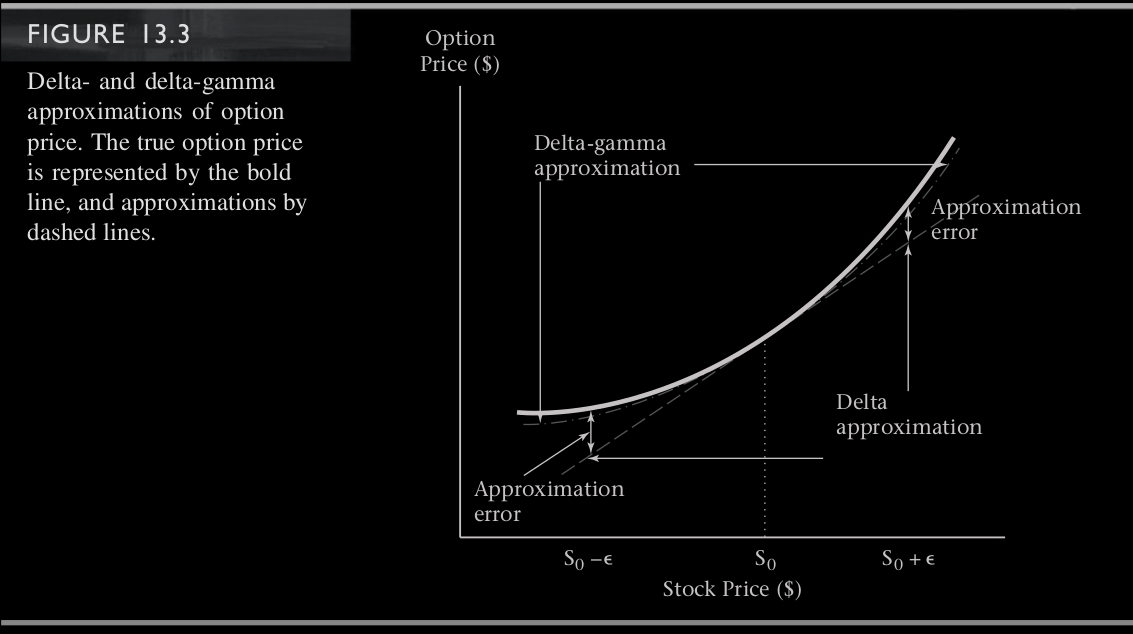
\includegraphics[scale=0.25]{figs/Figure_13-3.png}
\end{center}
\end{frame}
%-------------- end slide -------------------------------%}}}
%-------------- start slide -------------------------------%{{{ 1 Table 13.4
\begin{frame}[fragile,t]
 \begin{myexample}
  Given the first column of the following table, filling the details of the rest entries:
  \begin{center}
    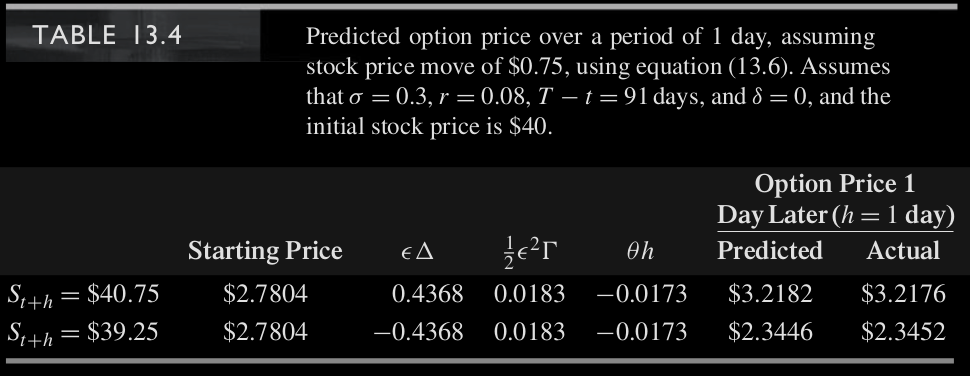
\includegraphics[scale=0.25]{figs/Table_13-4.png}
  \end{center}
 \end{myexample}
 \begin{mysol}
    Working with Mathematica code... \myEnd
 \end{mysol}
\end{frame}
%-------------- end slide -------------------------------%}}}
%-------------- start slide -------------------------------%{{{ 1 Market-maker's profit
\begin{frame}[fragile,t]
 \begin{center}
   The value of the market-maker's investment:\\
   \begin{align*}
     \Delta_t S_t -C(S_t)
   \end{align*}
   \vfill
   \mySeparateLine
   \vfill
   Market-marker's profit when the stock price changes \\
   by $\epsilon$ over a time interval $h$
   \bigskip
   \begin{align*}
     \underbrace{\Delta_t (S_{t+h}-S_t)}_{\text{Changes in value of stock}} -
     \underbrace{\left[C(S_{t+h})-C(S_t)\right]}_{\text{Changes in value of option}} -
     \underbrace{rh \left[\Delta_t S_t - C(S_t)\right]}_{\text{interest charge}}
   \end{align*}
 \end{center}
\end{frame}
%-------------- end slide -------------------------------%}}}
%-------------- start slide -------------------------------%{{{ 1 Simplification 1
\begin{frame}[fragile,t]
 \begin{center}
   Now replace $\underbrace{C(S_{t+h})-C(S_t)}_{\text{Changes in value of option}}$ by its second order approximation:

   \bigskip
   \begin{align*}
     C\left(S_{t+h}\right) - C(S_t)  \approx & \quad \Delta_t\times \left(S_{t+h}-S_t\right)                  \\
                                             & + \frac{1}{2} \times \Gamma_t \times\left(S_{t+h}-S_t\right)^2 \\
                                             & + h\times \theta_t
   \end{align*}
   \bigskip

   and $S_{t+h}-S_t$ by  $\epsilon$, we see that
 \end{center}
\end{frame}
%-------------- end slide -------------------------------%}}}
%-------------- start slide -------------------------------%{{{ 1 Simplification 2
\begin{frame}[fragile]
  \begin{gather*}
    \text{Market-maker's profit} \\ ||\\
     \underbrace{\Delta_t (S_{t+h}-S_t)}_{\text{Changes in value of stock}} -
     \underbrace{\left[C(S_{t+h})-C(S_t)\right]}_{\text{Changes in value of option}} -
     \underbrace{rh \left[\Delta_t S_t - C(S_t)\right]}_{\text{interest charge}} \\
     || \\
     -\left(\frac{1}{2}\epsilon^2 \Gamma_t + \theta_t h + r h \left[ \Delta_t S_t -C(S_t)\right]\right)
   \end{gather*}
\end{frame}
%-------------- end slide -------------------------------%}}}
%-------------- start slide -------------------------------%{{{ 1 Final step: self-financing
\begin{frame}[fragile,t]
 \begin{center}
   We have seen that the market-maker approximately breaks even for a one-standard-deviation move in the stock:\\
   \bigskip

  \begin{align*}
    \epsilon = \sigma S_t \sqrt{h} \qquad \Longleftrightarrow \qquad
    \epsilon^2 = \sigma^2 S_t^2 h
  \end{align*}

  \bigskip
  \mySeparateLine
  \bigskip

  Finally, we see that
  \bigskip

  \begin{gather*}
    \text{Market-maker's profit}                                                 \\ || \\
     \underbrace{\Delta_t (S_{t+h}-S_t)}_{\text{Changes in value of stock}} -
     \underbrace{\left[C(S_{t+h})-C(S_t)\right]}_{\text{Changes in value of option}} -
     \underbrace{rh \left[\Delta_t S_t - C(S_t)\right]}_{\text{interest charge}} \\ || \\
     -\left(\frac{1}{2}\sigma^2 S_t^2 \Gamma_t + \theta_t + r \left[ \Delta_t S_t -C(S_t)\right]\right)h
   \end{gather*}
 \end{center}
\end{frame}
%-------------- end slide -------------------------------%}}}
